% ===============================
% Chapter 1 - Introduction
% ===============================

\chapter{Introduction}
\label{chap:intro}

\noindent Artificial intelligence has become deeply integrated into modern life, with natural language processing (NLP) enabling computers to understand and generate human language~\cite{hirschberg2015advances}. Recent large language models (LLMs) such as GPT-3 and GPT-4 can produce coherent, context-aware text across many domains~\cite{brown2020gpt3, openai2023gpt4}, influencing education, healthcare, and online communication.

\smallskip
\noindent However, while LLMs excel at linguistic fluency, they often lack emotional intelligence (EI) the capacity to recognize and respond appropriately to human emotions~\cite{salovey1990emotional, goleman1995ei}. This limitation is critical in contexts where users seek empathy or emotional support~\cite{fitzpatrick2017woebot, larsen2022ai}.

\smallskip
\noindent This research explores how retrieval-augmented prompting and adaptive few-shot learning can improve the emotional sensitivity of LLMs, developing interpretable, emotion-aware systems that enhance trust and safety in human--AI interaction~\cite{demszky2020goemotions, zhou2023emotional}.

\smallskip
\noindent Before presenting the technical aspects of this research, it is important to highlight the context in which the project was carried out. The capstone was conducted in collaboration with \textit{Datadoit}, a technology-driven company that provided both the industrial environment and practical perspective necessary to frame the problem. Understanding the host company’s mission, objectives, and areas of expertise helps clarify how the academic research aligns with real-world challenges and why emotion recognition was considered a valuable area of exploration in this setting.  
\section{Company Description}
Datadoit\cite{datadoit} is a Data Analytics as a Service (DAaaS) provider that enables businesses to manage their analytics solutions effectively. Using a cloud-based response engine platform, it offers real-time access to analytical data. Combining expertise in Big Data and machine learning with a deep understanding of contemporary business challenges, DaTaDoIt helps its partners develop highly personalized and innovative analytical solutions. This allows clients to benefit from a variety of collaborations tailored to their specific data analysis needs. The official logo of the company is shown in the following Figure \ref{fig:datadoit_logo}.

\begin{figure}[htbp]
    \centering
    
\includegraphics[width=0.5\linewidth]{Images/Datadoitlogo (2).png}
    \vspace{0.5cm}
    \caption{Datadoit Logo.}
    \label{fig:datadoit_logo}
\end{figure}

\section{Goals and Objective of the Company}

DataDoIt aims to enhance its data management capabilities by focusing on collecting data from both internal and external sources, integrating and aggregating diverse data types, establishing data lakes, and implementing robust data governance policies to ensure high quality and sustainability of analytical projects. In the field of analytical services, DataDoIt is committed to delivering high-quality results through flexible Service Level Agreements (SLAs) that reflect a strong commitment to partner data. The company employs advanced techniques such as R\cite{Rsoftware} and Python\cite{python3} scripts for data cleaning pipelines and leverages its expertise in various development and benchmarking tools for machine learning to extract actionable insights that meet its partners' high expectations. Furthermore, DataDoIt provides real-time analysis solutions through its Data Analytics as a Service (DaaS) offerings, enabling the rapid deployment of analytical solutions and ensuring suitable access channels for clients. The company's VPS response engine generates and delivers real-time information for self-analysis requests, empowering clients with timely and accurate data for informed decision-making.\\

\noindent DataDoIt's core areas of focus, as illustrated in Figure  \ref{fig:datadoit_focus}, include Data Science, Machine Learning (ML), Deep Learning (DL), Edge AI, IoT \& Analytics, and Industry 4.0. These areas represent the company's commitment to leveraging cutting-edge technologies to provide comprehensive and innovative solutions across various industry sectors.

\begin{figure}[htbp]
    \centering
    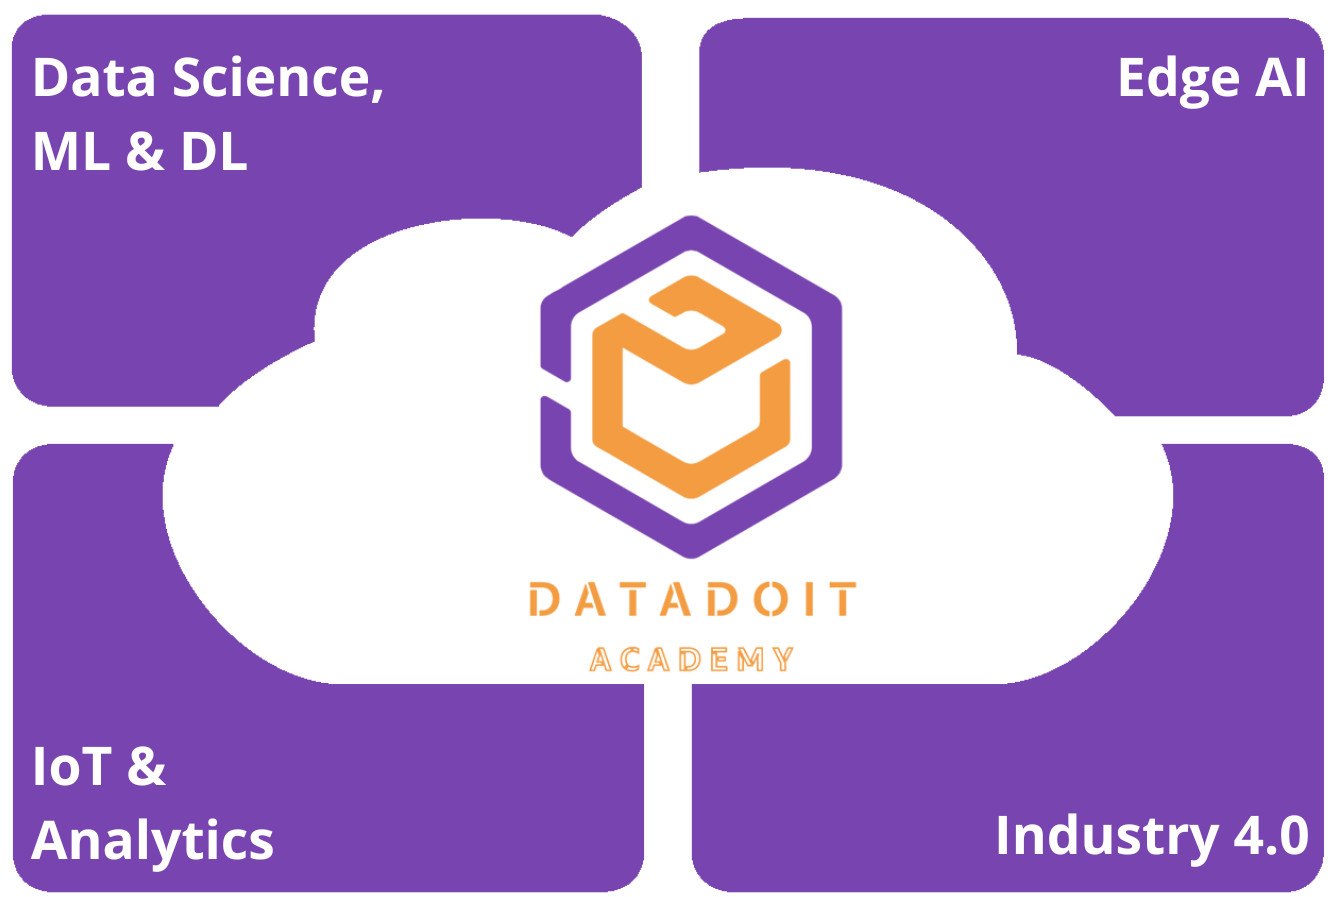
\includegraphics[width=0.4\linewidth]{Images/DataDoit.png}
     \vspace{0.5cm}
    \caption{DataDoIt Core Areas of Focus}
    \label{fig:datadoit_focus}
\end{figure}
\section{Project Context} 
 
Emotions shape how people communicate, make decisions, and interpret messages. In text-based communication, emotions remain present but often subtle, making emotion recognition both challenging and essential in today's digital world.
 
\noindent This challenge matters across multiple domains. Online platforms need emotion detection to foster supportive interactions. Customer service benefits from empathetic responses. Educational systems can adapt to student needs. Mental health applications can provide timely support.
\smallskip 
 
\noindent However, text-based emotion recognition is inherently difficult. Without vocal tone, facial expressions, or gestures, the same words can convey sincerity, sarcasm, or hostility depending on context.
\smallskip 
 
\noindent This project explores how emotions in text can be better recognized through layered analysis stages, reflecting how humans naturally interpret emotional meaning. It addresses both the technical challenge of building emotion recognition systems and the human need for understanding in digital communication.
\smallskip

\section{Problem Statement}

To protect vulnerable populations such as children, adolescents, and individuals facing mental health challenges, it is essential to ensure that Large Language Models (LLMs) can recognize and respond to emotions responsibly. Many people now rely on AI systems for support, advice, or companionship, but current models are not designed to reliably detect subtle emotional cues. A wrong interpretation can lead to dismissive or even harmful responses, especially in sensitive situations.  

\noindent The difficulty lies in the complexity of emotions and the limitations of text-based communication. Without tone, gestures, or expressions, the same phrase can mean very different things depending on context. While advanced models such as GPT-4 and other transformers show promise, they often struggle with nuanced distinctions and still operate as “black boxes,” offering little explanation for their choices.  

\noindent These challenges highlight the urgent need to systematically test existing LLMs for their emotional intelligence. This project addresses the problem by evaluating how well LLMs recognize emotions across different levels of granularity and by designing methods that make their reasoning more transparent and reliable.  

\begin{quote}
\textit{Illustrative Example:} Consider a mental-health chatbot interacting with a distressed user who writes, 
\textit{“I’m fine, just tired of everything.”} 
A conventional LLM may interpret this literally and respond with neutral advice, 
while an emotionally intelligent model identifies underlying sadness and adapts its tone empathetically. 
This simple case highlights the societal importance of reliable emotion recognition in text.
\end{quote}


\section{Pupose Of the Study}
The purpose of this study is to develop and evaluate a clear, human-centered approach to Emotion Recognition in Text  that reduces misunderstandings and supports safer, more empathetic interaction in digital settings. Rather than treating emotion recognition as a one-step label assignment, the study frames it as a \textit{multi-stage}, cognitively inspired process that mirrors how people naturally make sense of feelings in language. By doing so, the work aims to reveal where current tools are reliable, where they fail, and why those failures occur especially in subtle, high-stakes situations where the same words can carry very different meanings. The emphasis is practical: produce a transparent process that helps systems interpret emotional cues more responsibly and makes their reasoning easier to understand and improve.
\smallskip
\noindent A central motivation is the rapid adoption of LLM's systems trained to generate and interpret text which can appear fluent yet still misread emotions when context is thin, irony is present, or cultural cues are involved. This matters most when vulnerable users are involved, such as children, people in distress, or individuals seeking support, where a mistaken reading could lead to responses that are unhelpful or even harmful. The study therefore seeks to identify which parts of the emotion-understanding process LLMs handle well and which parts require safeguards, additional context, or human oversight. In concrete terms, the goal is to produce a structured pipeline, clear evaluation criteria, and practical guidance that together improve consistency, reduce risks of misinterpretation, and move ET closer to the way humans actually understand one another.
\section{Research Objectives}
This research is guided by three core objectives. They are formulated to provide both a methodological roadmap and a human-centered justification for the study. Together, these objectives define the steps through which the work is developed and evaluated, ensuring that improvements in technical performance also contribute to safer and more empathetic human–AI interaction.  

\textbf{Objective 1: Data Engineering.}  
To prepare and structure the dataset for emotion recognition by cleaning, organizing, and balancing the text examples so they can be used effectively in the study. High-quality, reproducible datasets form the foundation of reliable emotion recognition, ensuring that subsequent results are not distorted by noise or imbalance and that vulnerable users are not put at risk due to biased or incomplete training data.  

\textbf{Objective 2: Context Learning.}  
To examine how Large Language Models (LLMs) use contextual demonstrations (few-shot examples) to improve their ability to recognize emotions in text, especially in interactions with vulnerable users. Without adequate context, models may collapse subtle distinctions such as confusing sadness with disappointment or annoyance with anger leading to responses that are dismissive or harmful. By systematically varying the amount of context provided, this objective investigates how in-context learning helps LLMs distinguish nuanced affective states and thereby supports safer, more empathetic, and trustworthy responses.  

\textbf{Objective 3: Hybrid Semantic Analysis.}  
To design and evaluate a combined retrieval-guided prompting approach that integrates both lexical similarity (e.g., BM25) and semantic embeddings to strengthen emotion recognition. By ensuring that demonstrations are not only sufficient in quantity but also relevant in quality, this objective addresses the risk of misinterpretation when users express complex or ambiguous emotions. The hybrid approach is expected to yield more stable and interpretable outputs, contributing to human-centered safeguards where accurate emotional understanding is critical for responsible deployment of LLMs.  
\section{Research Questions}
To guide this research, three research questions were developed. Each question addresses a key challenge in the project and together they provide a clear direction for the research. They move from preparing the data, to exploring the role of context, and finally to testing a combined approach.

\noindent\textbf{Research Question 1:} How can the emotional intelligence of LLMs be detected and measured, particularly by examining the correlation between input text and predicted emotional output?  

\textbf{Rationale:} Detecting emotional intelligence depends on well-prepared data that ensures reliable input–output evaluation by focusing on data quality, this question aims to establish a solid foundation for assessing how well LLMs can recognize emotions in text.

\noindent\textbf{Research Question 2:} How does providing different levels of context improve the ability to understand emotions in text?  

\textbf{Rationale:} The meaning of emotions often depends on surrounding context. Without background information, the same words can be interpreted in very different ways.Studying context helps to see how much information is needed for accurate understanding.  

\noindent\textbf{Research Question 3:} How can a combined approach that blends different methods lead to more reliable and interpretable results?  

\textbf{Rationale:} A single method often misses important details. By combining different approaches, it may be possible to capture emotions more consistently and provide clearer explanations. This is especially important in sensitive applications where mistakes can have serious effects.  
\section{Approach and Boundaries of the Study}

This study follows a structured approach that combines methodological design with clearly defined boundaries. The approach outlines how the research is carried out, including the preparation of data, the exploration of context in learning, and the use of a hybrid analytical strategy. The boundaries clarify what is included and excluded from the study, ensuring that the work remains focused, manageable, and aligned with its goals. Together, the approach and boundaries provide a clear framework for how the study was conducted and the extent to which its findings can be applied.
\subsection{Scope}

This work looks at how emotions can be recognized in written text, since most of today’s communication happens through digital platforms. The study pays attention to how people express feelings in language and how this can be analyzed in a clear and structured way. It does not cover other forms of communication like speech, tone of voice, or body language, because the focus is on text alone.  

The scope of the project is also linked to real situations where understanding emotions matters, such as online conversations, learning environments, and mental health support. The aim is not to design finished products but to build knowledge that shows how emotions in text can be better understood and tested in practice.  

\subsection{Limitations}
\begin{itemize}
    \item Limitation 1: Dependence on publicly available datasets, which may not fully capture cultural and contextual diversity in emotional expression.  
    \item Limitation 2: Variation in the performance of large language models, as outcomes differ by model size and training data.  
    \item Limitation 3: Focus only on textual communication, excluding non-verbal cues such as tone, gestures, or facial expressions.  
    \item Limitation 4: Evaluation constrained by resources, preventing exhaustive testing of all models and configurations.  
\end{itemize}

\subsection{Delimitations}
\begin{itemize}
    \item Delimitation 1: Use of a recognized benchmark dataset to ensure comparability of results.  
    \item Delimitation 2: Focus on a selected set of large language models and methods to maintain clarity.  
    \item Delimitation 3: Exclusive attention to text-based emotion recognition to provide depth in one modality.  
    \item Delimitation 4: Concentration on three directions data engineering, context learning, and hybrid analysis rather than exploring every possible method.  
\end{itemize}


\subsection{Assumptions}

\begin{itemize}
    \item Assumption 1: The dataset is sufficiently representative of common emotional expressions.  
    \item 
    \textit{Rationale:} The GoEmotions dataset is one of the largest and most widely cited benchmarks in the field, making it a reasonable basis for testing.  

    \item Assumption 2: Providing contextual examples to large language models improves their ability to interpret emotions in text.  
    \item 
    \textit{Rationale:} Prior studies on few-shot learning have shown that examples guide model reasoning, and this research builds on that principle to test emotional understanding.  
\end{itemize}

\subsection{Expected Contributions}
The main contributions of this study can be summarized as follows:
\begin{itemize}
    \item Application of the \textbf{Design Science Research (DSR) methodology} to structure the research process and ensure systematic development and evaluation.  
    \item Development of a structured data engineering process that prepares and balances textual data for reliable experimentation.  
    \item Examination of how context learning (e.g., few-shot and n-shot approaches) influences the ability of large language models to interpret text.  
    \item Design and evaluation of a hybrid semantic analysis approach that combines embeddings with retrieval methods such as BM25.  
\end{itemize}
\newpage

\subsection{Structure of the Report}
The report is organized into chapters that follow a logical progression:
\begin{itemize}
    \item \hyperref[chap:intro]{\textbf{Chapter 1: Introduction}}   introduces the overall context of the study, explains why emotion recognition in text is important, and sets out the problem being addressed. It also presents the main goals, research questions, and the boundaries of the work.  
    
    \item \hyperref[chap:background]{\textbf{Chapter 2: Background and Literature Review}}   provides the theoretical and academic foundation of the project. It reviews existing studies on emotion recognition, large language models, and related methods, while highlighting the gaps that motivate this research.  
    
    \item \hyperref[chap:methodology]{\textbf{Chapter 3: Methodology}}   describes the research approach that was followed. It explains how the study was structured, the steps taken to ensure rigor, and the reasoning behind the chosen process.  
    
    \item \hyperref[chap:Iterations]{\textbf{Chapter 4: Iterations}}   outlines the development process through its different phases. Each iteration builds on the previous one, gradually shaping the final system and showing how the solution was refined step by step.  
    
    \item \hyperref[chap:results]{\textbf{Chapter 5: Results and Validation}}   presents the main findings of the study. It discusses what was achieved, how the results were evaluated, and what they reveal about the effectiveness of the proposed approach.

    \item \hyperref[chap:discussion]{\textbf{Chapter 6: Discussion}}   interprets the results in depth, situates them within existing literature, and discusses their practical implications, limitations, and future directions.

    \item \hyperref[chap:conclusion]{\textbf{Chapter 7: Conclusion}}   summarizes the overall contributions of the work. It reflects on the significance of the findings, acknowledges limitations, and points to possible directions for future research.
\end{itemize}   